\documentclass[12pt,a4paper]{article}
\usepackage[utf8]{inputenc}
\usepackage[german]{babel}
\usepackage[T1]{fontenc}
\usepackage{amsmath}
\usepackage{amsfonts}
\usepackage{amssymb}
\usepackage{graphicx}
\usepackage{float}
\usepackage[left=2cm,right=2cm,top=2cm,bottom=2cm]{geometry}
\author{Tim}

\begin{document}
\setlength{\parindent}{0pt} 
\begin{center}
{\LARGE Versuchsprotokoll}\\
\begin{large}
zum Grundpraktikum Physik Teil I\\[0.4cm]
an der RWTH Aachen\\
I. Physikalisches Institut B\\[4.5cm]
\Large\textbf{\textsl{Thermodynamik}}\\[4cm]
\normalsize\textit{vorgelegt\\von}\\[0.4cm]
\large{Moritz Berger\\Tim Herbermann\\Gerald Kolter\\Sebastian Siebert}\\[1cm]
\large \textit{Gruppe B07} \\ [3cm]
\large \textbf{Wintersemester 2016/2017}
\end{large}
\end{center}
\newpage
\tableofcontents
\newpage

\section{Versuchsbeschreibung}
Ziel des Versuches ist die Vermessung der Dampfdruckkurve und die Bestimmung der Verdampfungsenthalpie von Wasser.\\

\subsection{Dampfdruckkurve}
In diesem Versuch soll nur der Übergang zwischen dem flüssigen und gasförmigen Aggregatzustand betrachtet werden. \\
In einer Flüssigkeit in einem evakuiertem, abgeschlossenem Gefäß verdampfen und kondensieren die Moleküle bis sich ein Gleichgewicht einstellt. Der Druck des Dampfes ist von der Temperatur und der Flüssigkeit abhängig und wird als Dampfdruck oder Sättigungsdruck bezeichnet. Der Zusammenhang von Sättigungsdampfdruck und Temperatur wird als Dampfdruckkurve bezeichnet. Wäre das Gefäß nicht evakuiert, würde sich das Gleichgewicht langsamer einstellen, der Dampfdruck wäre allerdings der gleiche, da die Partialdrücke einzelner Gase von der Anwesenheit anderer Gase nicht beeinflusst werden.

\subsection{Verdampfungsenthalpie}
Die Verdampfungsenthalpie beschreibt, wie viel Energie notwendig ist, um ein Mol des jeweiligen Stoffs (in diesem Fall Wasser) zu Verdampfen. Führt man einer gewissen Menge flüssigem Wasser langsam immer mehr Wärmeenergie zu und misst dabei die Temperatur, so ist die Verdampfungsenthalpie als Plateau beobachtbar. Trotz des Zuführens weiterer Wärmeenergie ändert sich die Temperatur nicht. \\

Der Sättigungsdampfdruck wird quantitativ durch die Clausius-Clapeyron-Gleichung beim Phasenübergang flüssig-gasförmig beschrieben.

\begin{equation}
\frac{dp}{dT}=\frac{\nu \Lambda}{T(V_{gas}-			V_{fl"ussig})}
\end{equation}

Da $V_{gas} >> V_{fl"ussig}$ folgt unter der Annahme das sich die Verdampfungsenthalpie $\Lambda$ innerhalb von kleinen Temperaturbereichen nicht ändert mittels Integration den für diesen Versuch entscheidenden Zusammenhang:

\begin{equation}
\ln{(p/p_0)}=-\frac{\Lambda}{R} \left(\frac{1}{T}-			\frac{1}{T_0}\right)
\end{equation}

Mit diesem Zusammenhang kann die Verdampfungsenthalpie $\Lambda$ für verschiedene Temperaturen bestimmt werden, indem um diese Punkte innerhalb kleiner Temperaturänderungen eine Gerade angepasst wird.
\newpage
\section{Aufbau und Durchführung}
\label{sec:Aufbau und Durchfühung}

\subsection{Aufbau}

\begin{figure}[H]
\includegraphics[width=\linewidth]{Bilder/AufbauB}
\caption[AufbauB]{Aufbau}
\label{fig:AufbauB}
\end{figure}

Der Glaskolben wird etwa zur Hälfte mit Wasser gefüllt und über die entsprechenden Anschlüsse mit Temperaturfühler und Drucksensor verbunden. Sowohl der Kolben als auch die Messinstrumente werden am Stativ befestigt. Der Heizpilz wird auf dem ausgefahrenen Laborheber so unter den Kolben montiert, dass er schnell entfernt werden kann. Eine Handvakuumpumpe wird über den Dreiwegehahn mit dem Kolben verbunden. Der Aufbau ist in Abbildung \ref{fig:AufbauB} gezeigt.\\
Das Thermometer wird über die Thermobox und der Drucksensor direkt über die Anschlüsse mit dem CASSY verbundenen. Die Einstellungen finden sich in Tabelle \ref{tab:CASSY}. \\

\begin{table}[H]
\begin{center}
\begin{tabular}{|c|c|c|c|}
\hline
- & Messbereich & Messintervalle & Anzahl Messwerte\\
\hline
Drucksensor & 0hPa bis 1500hPa& 1s & 300\\
\hline
Temperaturfühler & -20C bis 120C& 1s & 300\\
\hline
\end{tabular}
\caption{Einstellungen CASSY}
\label{tab:CASSY}
\end{center}
\end{table}

Falls nicht anders vermerkt, wurden immer diese Einstellungen verwendet.

\subsection{Durchführung}

Um eine aussagekräftige Hauptmessung durchführen zu können ist es nötig die Messgeräte zu kalibrieren sowie den Fehler auf die Messung abzuschätzen. Dazu werden entsprechende Kalibrierungsmessungen und Rauschmessungen durchgeführt.\\

%hier ggf. ausführlicher werden!
Die Rauschmessung des Drucksensors wird zusammen mit der Kalibrierung des Temperaturfühlers durchgeführt. Dazu werden für etwa $300s$ Messwerte aufgezeichnet.\\
Zur Überprüfung der Gasdichtigkeit wird mit der Handvakuumpumpe bei verschlossenem Auslass der Druck im Glaskolben unter $200hPa$ gesenkt und der zeitliche Verlauf des Drucks gemessen. Aus dem Anstieg des Druckes kann die Undichtigkeit des Aufbaus bestimmt werden. Die Druckveränderung sollte nach Möglichkeit nicht $0,2 \dfrac{mbar}{min}$ übersteigen damit eine vernachlässigbare Undichtigkeit erreicht ist. \\

Im Hauptversuch wird bei geöffnetem Auslass das Wasser im Glaskolben bis zum Sieden erhitzt. Hat man sich davon überzeugt das der Kolben keine Luft mehr enthält wird der Auslass geschlossen, der Heizpilz entfernt und die Messung gestartet. Während des Abkühlens wird dann die Dampfdruckkurve aufgezeichnet bis das Wasser im Kolben aufhört zu sieden.\\
Am Ende des Messvorgangs lässt man das Wasser weiter bis auf Raumtemperatur abkühlen und führt gegebenenfalls eine zweite Dichtigkeitsmessung durch, um sich davon zu überzeugen, dass die Undichtigkeit des Aufbaus während des Versuchs nicht gestiegen ist. 

\section{Versuchsauswertung}
Der Versuch wurde von zwei Teilgruppen unabhängig voneinander durchgeführt. Im folgenden werden diese mit \glqq Versuch A \grqq und \glqq Versuch B \grqq bezeichnet und nebeneinander ausgewertet.

\subsection{Rauschmessung}

\begin{figure}[H]
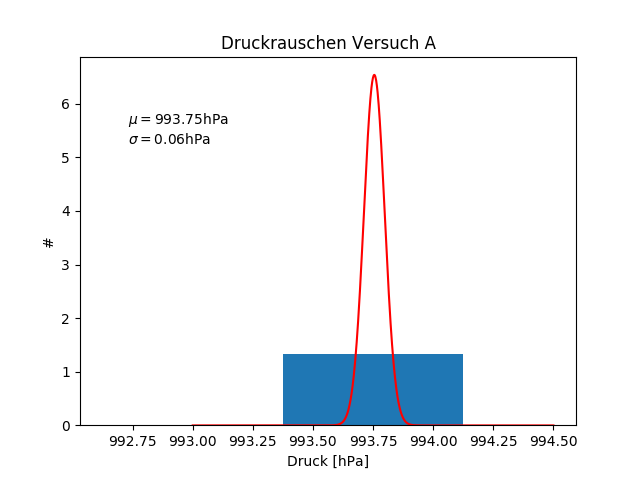
\includegraphics[scale=0.5]{Bilder/DruckrauschenA}
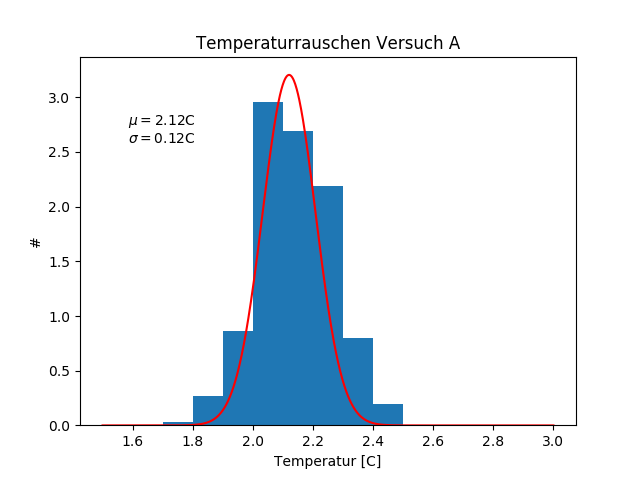
\includegraphics[scale=0.5]{Bilder/TemprauschenA}
\caption[Rauschen Versuch A]{Rauschmessung des Drucksensors (links) und des Temperaturfühlers (rechts). Eine Gaußkurve mit entsprechenden Parametern ist zusätzlich eingezeichnet.}
\label{fig:RauschenA}
\end{figure}

\begin{table}[H]
\begin{center}
\begin{tabular}{|c|c|c|}
\hline
- & $\mu$ & $\sigma$\\
\hline
Druck & 993.75 & 0.22\\
\hline
Temperatur & 2.12 & 0.12\\
\hline
\end{tabular}
\caption[Tab. Rauschen A]{Ergebnisse der Rauschmessungen für Versuch A}
\label{tab:RauschenA}
\end{center}
\end{table}

Die Ergebnisse der Rauschmessungen für Versuch A sind in Abb. \ref{fig:RauschenA} und Tab. \ref{tab:RauschenA} dargestellt.\\
Dabei wurde der Fehler auf das Druckrauschen durch eine Gleichverteilung bestimmt:
\begin{equation}
\sigma_p =\dfrac{0.75hPa}{\sqrt{12}} = 0.22hPa
\end{equation}

Der Fehler auf die Temperatur folgt aus der Gaußverteilung als Standardabweichung.






\begin{figure}[H]
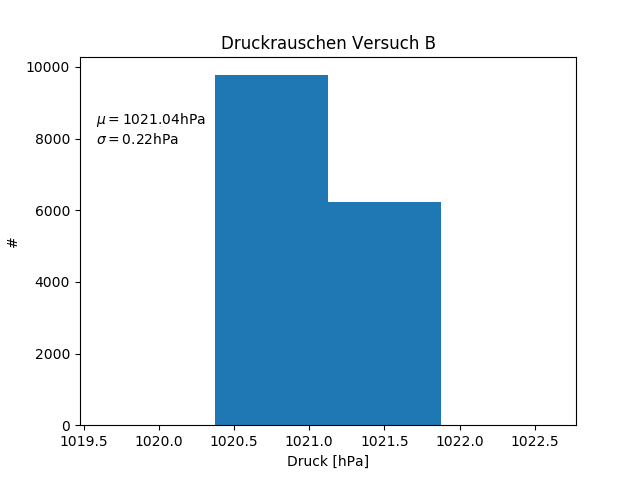
\includegraphics[scale=0.5]{Bilder/DruckrauschenB}
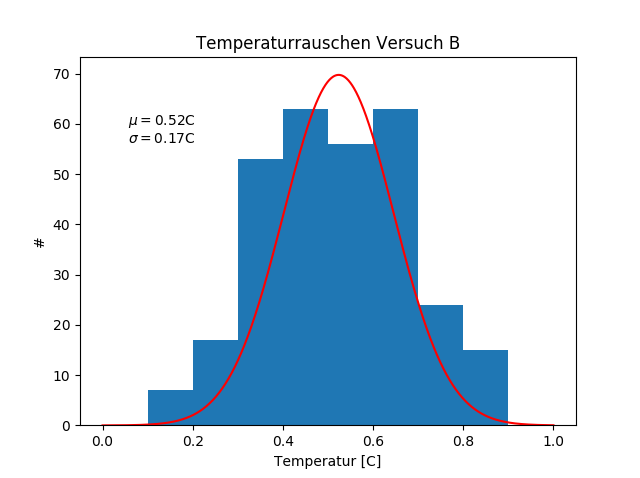
\includegraphics[scale=0.5]{Bilder/TemprauschenB}
\caption[Rauschmessung Versuch B]{Rauschmessung des Drucksensors (links) und des Temperaturfühlers (rechts) für B.}
\label{fig:RauschenB}
\end{figure}


\begin{table}[H]
\begin{center}
\begin{tabular}{|c|c|c|}
\hline 
- & $\mu$ & $\sigma$\\ 
\hline 
Temperatur[C] & 22.99 & 0.17 \\ 
\hline 
Druck[hPa] & 1021.04 & 0.22\\ 
\hline 
\end{tabular}
\caption[Tabelle Rauschenmessung B]{Ergbenisse der Rauschmessung für Versuch B}
\label{tab:RauschenB}
\end{center}
\end{table}

Die Ergebnisse der Rauschmessungen für Versuch B finden sich in Abb. \ref{fig:RauschenB} und Tab. \ref{tab:RauschenB}. Die Fehler ergeben sich dabei durch völlig analoges Vorgehen zu Versuch A.



\subsection{Kalibrierung der Sensoren}

Bei jeweils 0C und Siedetemperatur wurde eine Rauschmessung der Temperatur durchgeführt. Da am Versuchstag nicht Normaldruck, sondern ein Druck von 1005hPa geherrscht hat, muss die Siedetemperatur noch auf 99.72C korrigiert werden. Die Ergebnisse sind in Tabelle \ref{tab:KaliA} aufgeführt. Die angegebenen Fehler sind die Fehler des Mittelwertes.

\begin{table}[H]
\begin{center}
\begin{tabular}{|c|c|}
\hline 
$T_{erwartet}[C]$ & $T_{gemessen}[C]$ \\ 
\hline 
$0$ & $2.121\pm0.007$ \\ %unterschiedliche Nachkommastellen? (punkt 7)
\hline 
$99.72$ & $99.39\pm0.01$ \\ 
\hline 
\end{tabular}
\caption[Ergebnisse Kalibrierungsmessung A]{Ergebnisse Kalibrierungsmessung A} 
\label{tab:KaliA}
\end{center}
\end{table}

Aus diesen Ergebnissen wird nun eine Ausgleichsgerade bestimmt (Abb.\ref{fig:GeradeKaliA}).

\begin{figure}[H]
\begin{center}
\centering
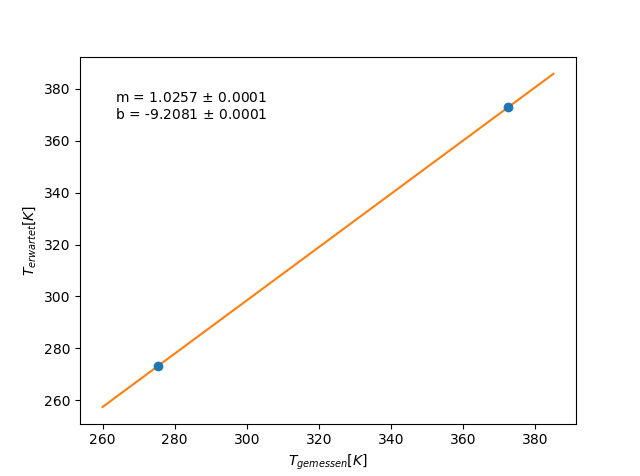
\includegraphics[width=0.9\linewidth]{Bilder/KalibrationA}
\caption[Gerade Kalibration A]{Ausgleichsgerade bei der Kalibration(VersuchA)\\
Anmerkung: Die Fehler auf den Mittelwerten sind sehr klein und deswegen hier nicht sichtbar.}
\label{fig:GeradeKaliA}
\end{center}
\end{figure}


Die Kalibrierung (Abb.\ref{fig:GeradeKaliA}) ergibt für die Steigung:
\begin{equation}
m = \dfrac{99.72K}{T_{Eis}-T_{siedend}} = 1.0257
\end{equation}

\begin{equation}
\sigma_{m} = m\cdot \sqrt{(\dfrac{\sigma_{T_{siedend}}\cdot 99.72K}{(T_{siedend}-T_{Eis})^{2}})^{2}+(\dfrac{\sigma_{T_{Eis}}\cdot 99.72K}{T_{siedend}-T_{Eis}})^{2}} = 0.0001
\end{equation}

\begin{equation}
b = 372.87K-m\cdot T_{siedend} = -9.20810K
\end{equation}

\begin{equation}
\sigma_{b} = \sqrt{(\dfrac{\sigma_{m}}{m})^{2}+(\dfrac{\sigma_{T_{siedend}}}{T_{siedend}})^{2}} = 0.0001K
\end{equation}

Damit können die wirklichen Temperaturen berechnet werden:

\begin{equation}
T_{erwartet}=1.0257\cdot T_{gemessen}-9.2081K
\end{equation}

Aus der Fehlerfortpflanzung folgt der (im Hauptversuch als systematisch betrachtete) Fehler auf die Temperatur:

\begin{equation}
\sigma_{T_{erwartet}} = \sqrt{(T_{gemessen} \cdot \sigma_m)^2 + (m \cdot \sigma_{T_{gemessen}})^2 + \sigma_b^2}
\end{equation}

%Wobei $\sigma_T = 0.12$ und eine Temperatur von 100C angenommen wurde.\\
%100C ?  und sigma_T=0.12? sollte das nicht der einzelwertfehler sein?
Durch analoges Vorgehen für Versuch B ergeben sich die in Tabelle \ref{tab:KaliB} dargestellten Ergebnisse. Die angegeben Fehler sind wieder die Fehler des Mittelwertes.


\begin{table}[H]
\begin{center}
\begin{tabular}{|c|c|}
\hline 
$T_{erwartet}[C]$ & $T_{gemessen}[C]$ \\ 
\hline 
$0$ & $0.52 \pm 0.01$ \\ 
\hline 
$99.72$ & $99.24\pm 0.005$ \\ %nachkommastellen
\hline 
\end{tabular}
\caption[Ergebnisse Kalibrierungsmessung B]{Ergebnisse Kalibrierungsmessung B}
\label{tab:KaliB}
\end{center}
\end{table}


\begin{figure}[H]
\centering
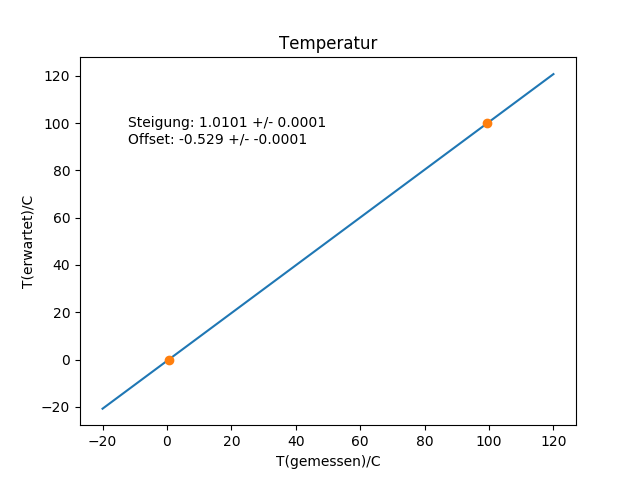
\includegraphics[width=0.9\linewidth]{Bilder/KalibrationB}
\begin{center}
\caption[KalibrationB]{Ausgleichsgerade bei der Kalibration (VersuchB)\\
Anm.: Die Fehler auf den Mittelwerten sind sehr klein und deswegen hier nicht sichtbar.}
\label{fig:GeradeKaliB}
\end{center}
\end{figure}


Die Kalibrierung (Abb.\ref{fig:GeradeKaliA}) ergibt für die Steigung:
\begin{equation}
m = \dfrac{99.72K}{T_{Eis}-T_{siedend}} = 1.0100
\end{equation}

\begin{equation}
\sigma_{m} = m\cdot \sqrt{(\dfrac{\sigma_{T_{siedend}}\cdot 99.72K}{(T_{siedend}-T_{Eis})^{2}})^{2}+(\dfrac{\sigma_{T_{Eis}}\cdot 99.72K}{T_{siedend}-T_{Eis}})^{2}} = 0.0001
\end{equation}

\begin{equation}
b = 372.87K-m\cdot T_{siedend} = -3.2664K
\end{equation}

\begin{equation}
\sigma_{b} = b\cdot \sqrt{(\dfrac{\sigma_{m}}{m})^{2}+(\dfrac{\sigma_{T_{siedend}}}{T_{siedend}})^{2}} = 0.0001K
\end{equation}


Damit können die wirklichen Temperaturen berechnet werden:
\begin{equation}
T_{erwartet}=1.01\cdot T_{gemessen}-3.2664K
\end{equation}
 
%Wobei $\sigma_T = 0.04$ und eine Temperatur von 100C angenommen wurde\\
%100C? 0.04 ist doch wieder einzelfehler und nicht mittelwert?

Für die Korrekturen am Drucksensor siehe Tabelle \ref{tab:Druckoffsets}.

\begin{table}
\begin{center}
\begin{tabular}{|c|c|c|}
\hline
Versuch & Steigung & Offset[C]\\
\hline
A & $1.0252 \pm 0.0001$ & $-2.1740 \pm 0.0003$\\
\hline
B & $1.0101 \pm 0.0001$ & $-0.5290 \pm 0.0001$\\
\hline
\end{tabular}
\end{center}
\caption{Zusammenfassung der Ergebnisse der Kalibrierung für A und B}
\label{tab:KaliErgebnisseAundB}
\end{table}


\begin{table}
\begin{center}
\begin{tabular}{|c|c|c|}
\hline
Versuch & Druck (gemessen)[hPa] & Offset [hPa]\\
\hline
A & $993.75 \pm 0.22$ & $11.25 \pm 0.22$\\
\hline
B & $1021.04 \pm 0.22$ & $-16.04 \pm 0.22$\\
\hline
\end{tabular}
\end{center}
\caption[Offsets]{Druckoffsets für A und B.}
\label{tab:Druckoffsets}
\end{table}







\subsection{Dichtigkeitsmessung}
Eine sehr wichtige Voraussetzung für sinnvolle Ergebnisse ist, dass die Messapparatur dicht ist. Die Daten aus dem in Abschnitt \ref{sec:Aufbau und Durchfühung} erklärten Messverfahren vor dem Hauptversuch und die zugehörigen Residuen sind für Aufbau A in Abbildung \ref{fig:DichtigkeitA} zu sehen. Das Muster, dass sich in den Residuen zeigt, ist bedingt durch das Auflösungsvermögen des Drucksensor, welches eindrucksvoll anhand der Stufenform des Plots der Rohdaten zu sehen ist. \\
Aufgrund der Leckrate von $(0,215 \pm 0,02) \dfrac{hPa}{min}$ kann die Apparatur als dicht angenommen werden und der gemessene Druck kann direkt verwendet werden und muss nicht korrigiert werden.\\
Auf eine Dichtigkeitsmessung nach dem Hauptversuch wurde verzichtet da während des Abkühlens der Aufbau empfindlich gestört wurde und keine Dichtigkeit mehr gegeben war. Es wird im weiteren Verlauf der Auswertung angenommen das die Undichtigkeit von Versuchsaufbau A während des Hauptversuchs vernachlässigbar klein blieb.

\begin{figure}
\centering
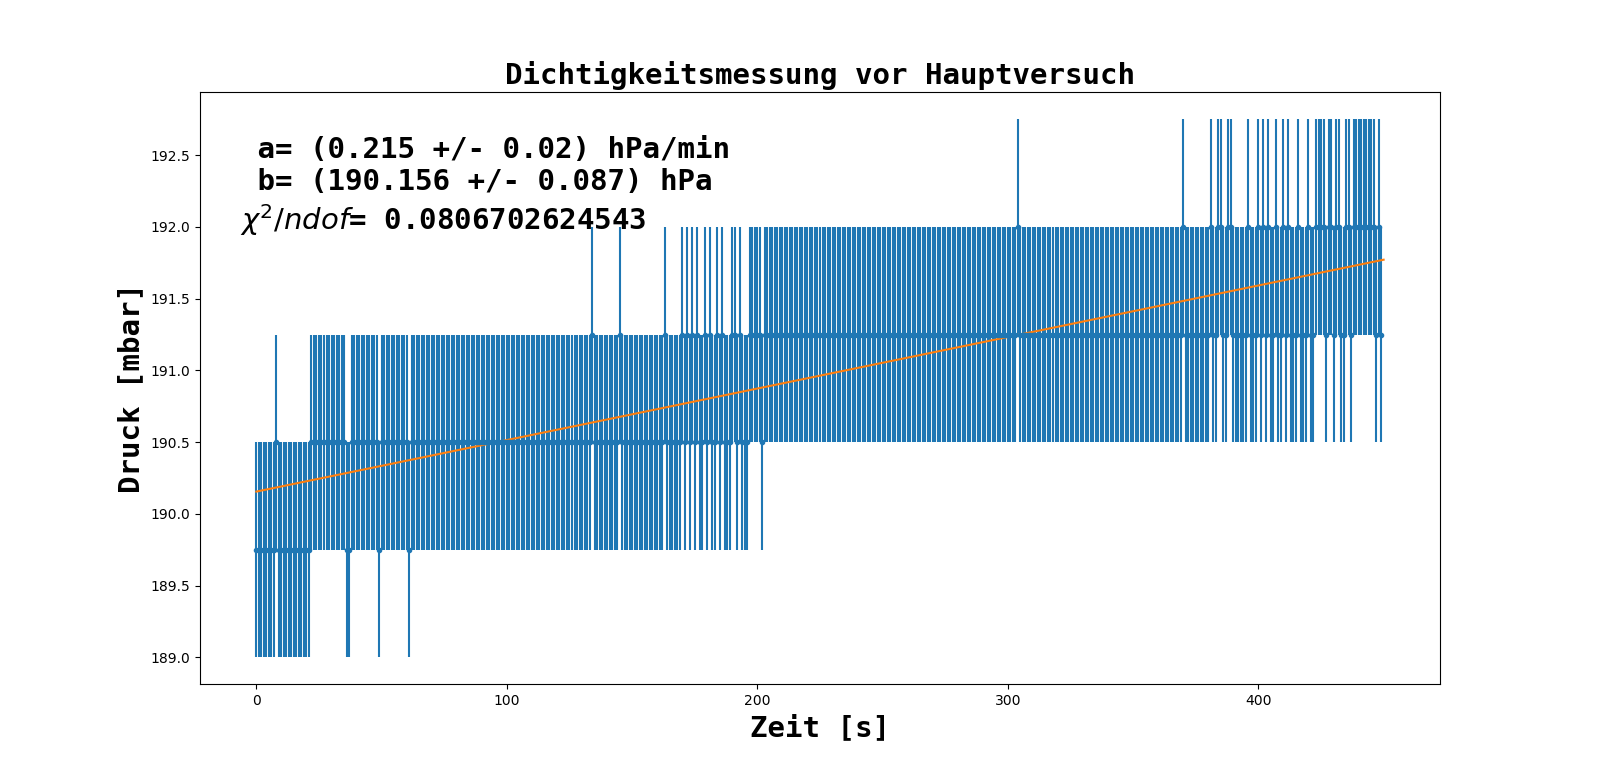
\includegraphics[width=\linewidth]{Bilder/Dichtigkeit_vorher_A.png}
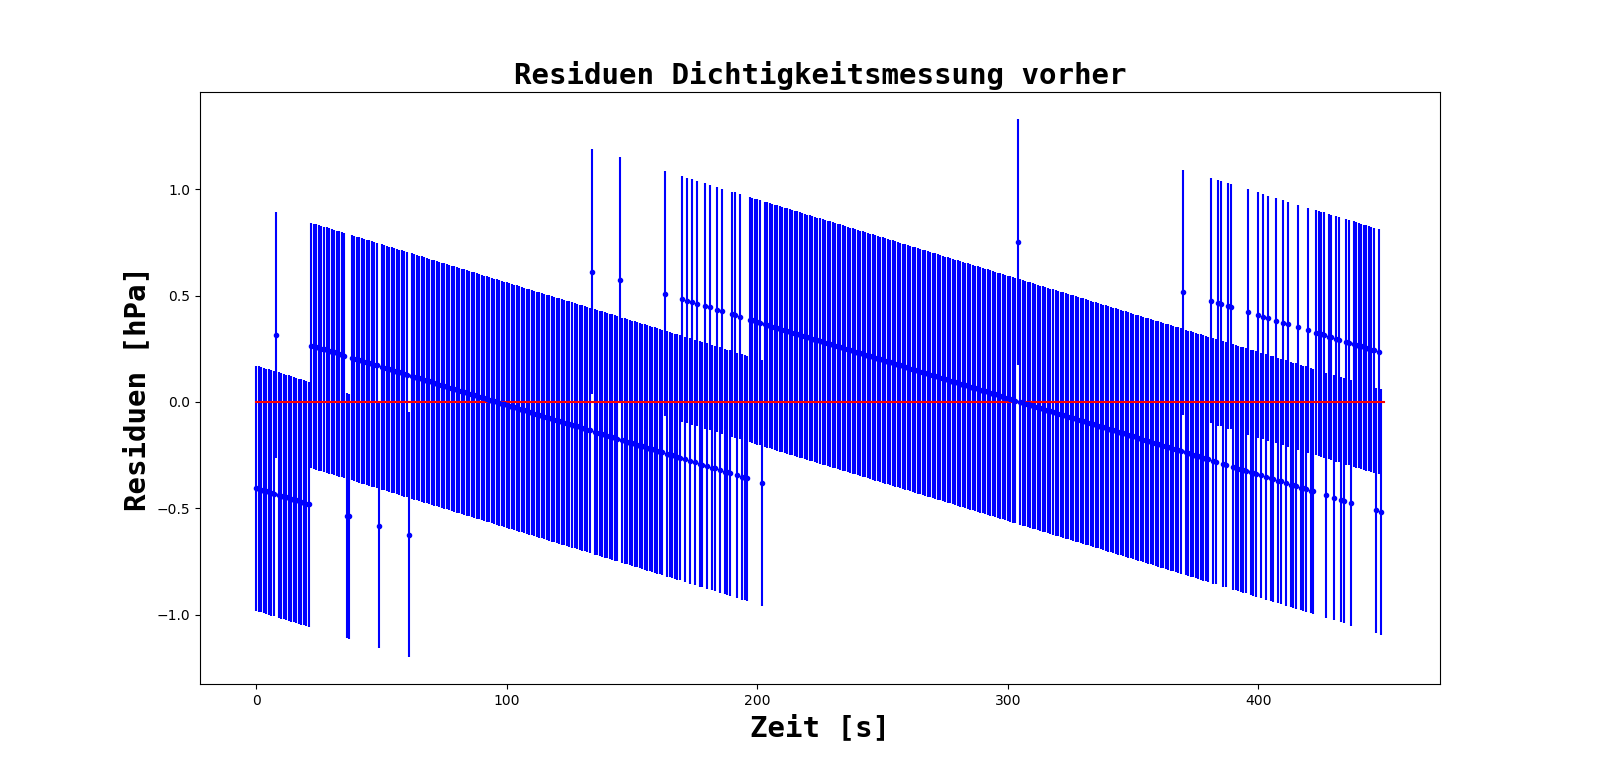
\includegraphics[width=\linewidth]{Bilder/Residuen_Dichtigkeit_vorher_A.png}
\caption[Dichtigkeit vor Hauptversuch Apparatur A]{Dichtigkeit vor Hauptversuch Apparatur A}
\label{fig:DichtigkeitA}
\end{figure}

Die Ergebnisse der Dichtigkeit für Aufbau B vor der Hauptmessung sind ähnlich und finden sich in Abbildung \ref{fig:DichtigkeitB}.\\
Aufgrund der Leckrate von $(0,236 \pm 0,035) \dfrac{hPa}{min}$ kann die Apparatur auch hier als dicht angenommen werden und der gemessene Druck kann direkt verwendet werden und muss nicht korrigiert werden.\\
Nach Durchführung des Hauptversuches wurde für Aufbau B eine erneute Dichtigkeitsmessung vorgenommen (Abb. \ref{fig:DichtigkeitNachherB}).\\
Die Leckrate ist mit $(2,718 \pm 0,160) \dfrac{hPa}{min}$ deutlich schlechter geworden im Vergleich zu der Leckrate vor dem Hauptversuch. Dies könnte daran liegen, dass die Dichtigkeitsmessung nicht mit dem nach dem Hauptversuch vorhandenen Unterdruck durchgeführt wurde, sondern wie zu Beginn mit der Handvakuumpumpe. Durch das Wackeln an der Apparatur beim Anschließen dieser könnten sich Undichtigkeiten aufgetan haben, welche dann den Wert der zweiten Messung verschlechtert haben, auf die Hauptmessung aber keinen Einfluss haben, weil sie erst nach dieser aufgetreten sind. Daher wird im Folgenden davon dennoch ausgegangen, dass die Undichtigkeit vernachlässigbar gering ist.


\begin{figure}
\centering
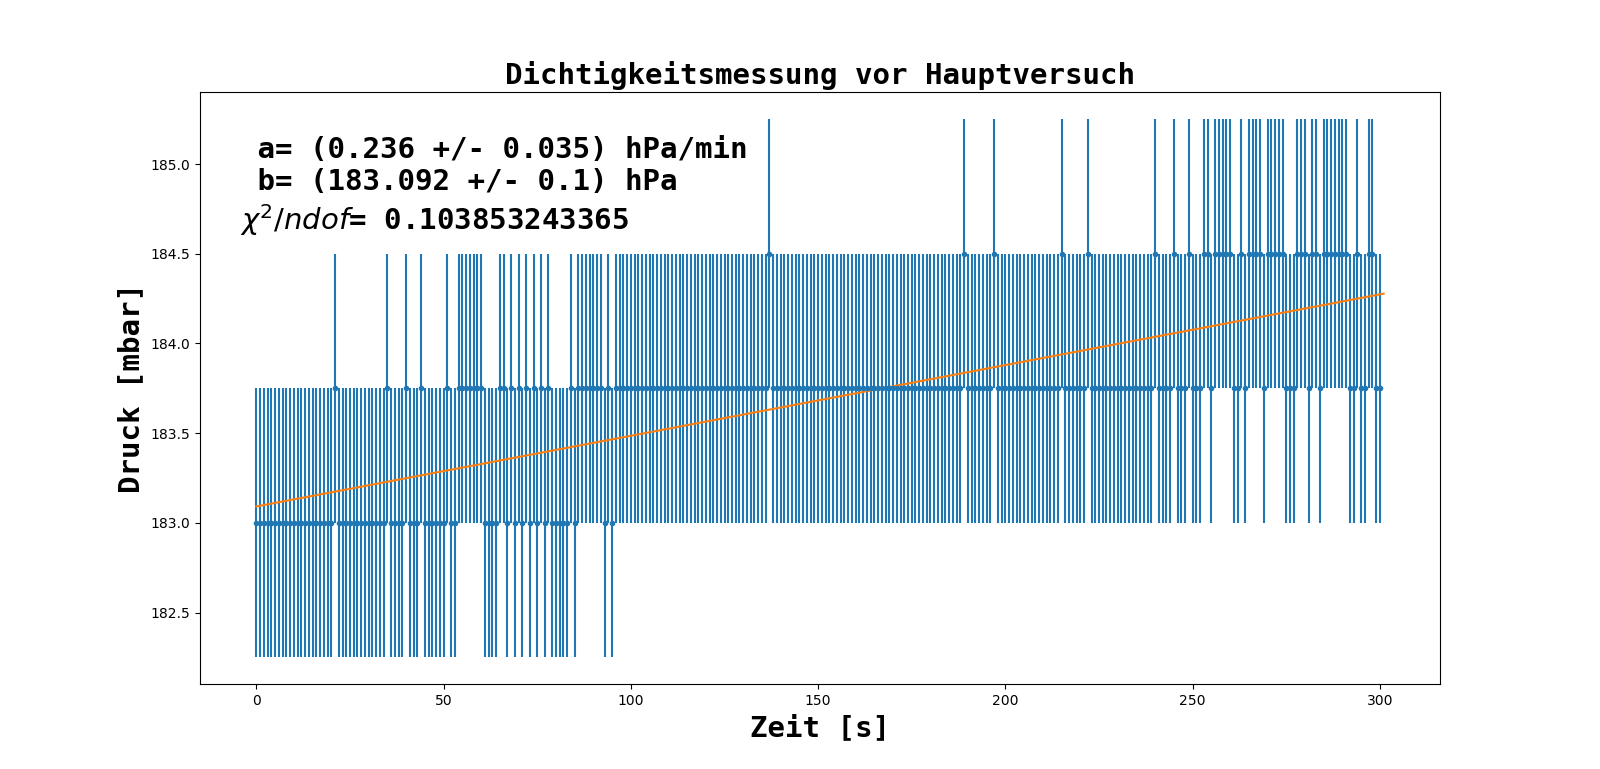
\includegraphics[width=\linewidth]{Bilder/Dichtigkeit_vorher_B.png}
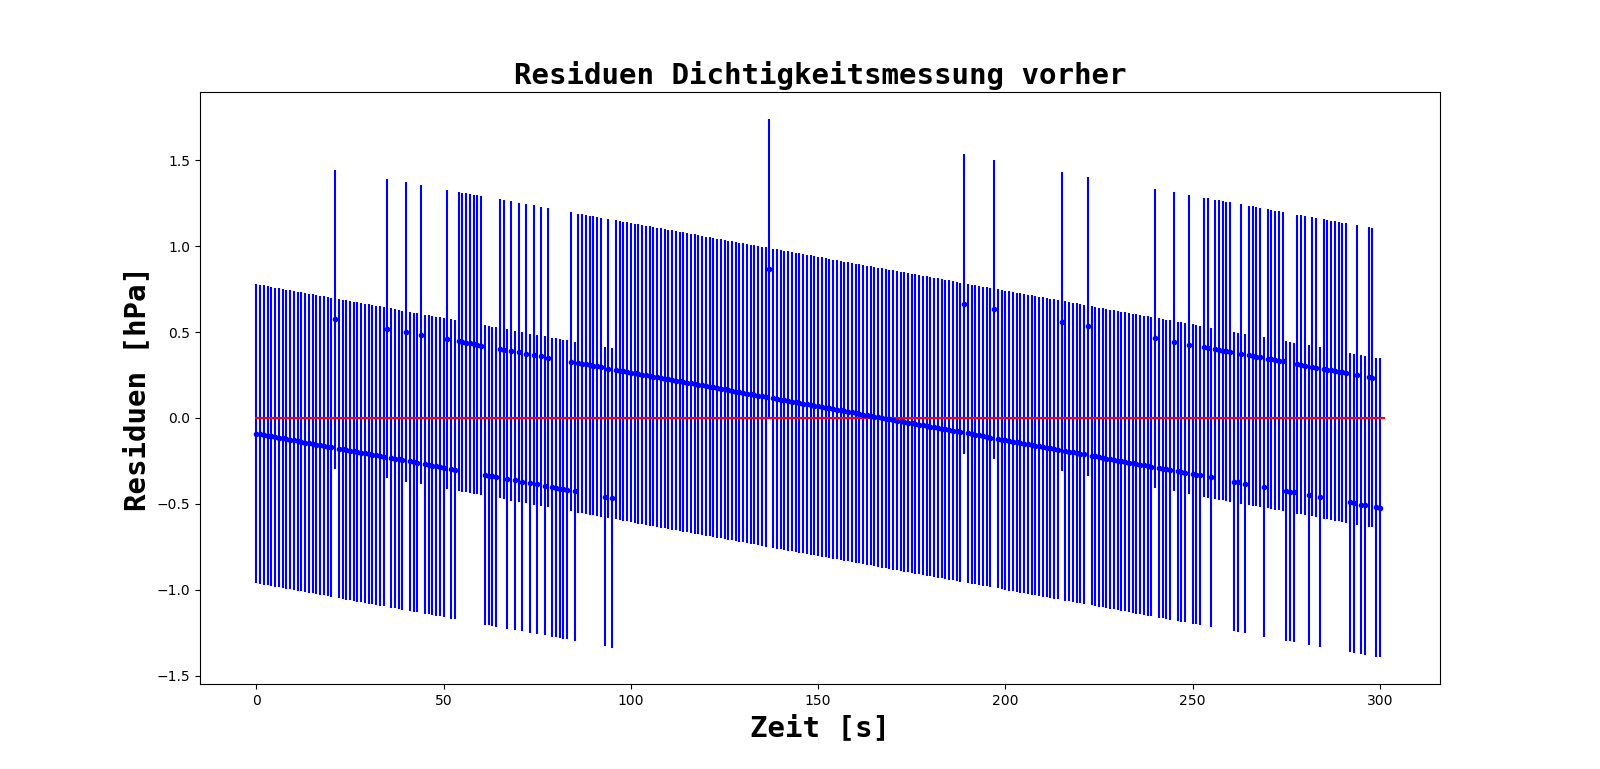
\includegraphics[width=\linewidth]{Bilder/Residuen_Dichtigkeit_vorher_B.png}
\caption[Dichtigkeit vor Hauptversuch Apparatur B]{Dichtigkeit vor Hauptversuch Apparatur B}
\label{fig:DichtigkeitB}
\end{figure}

\begin{figure}
\centering
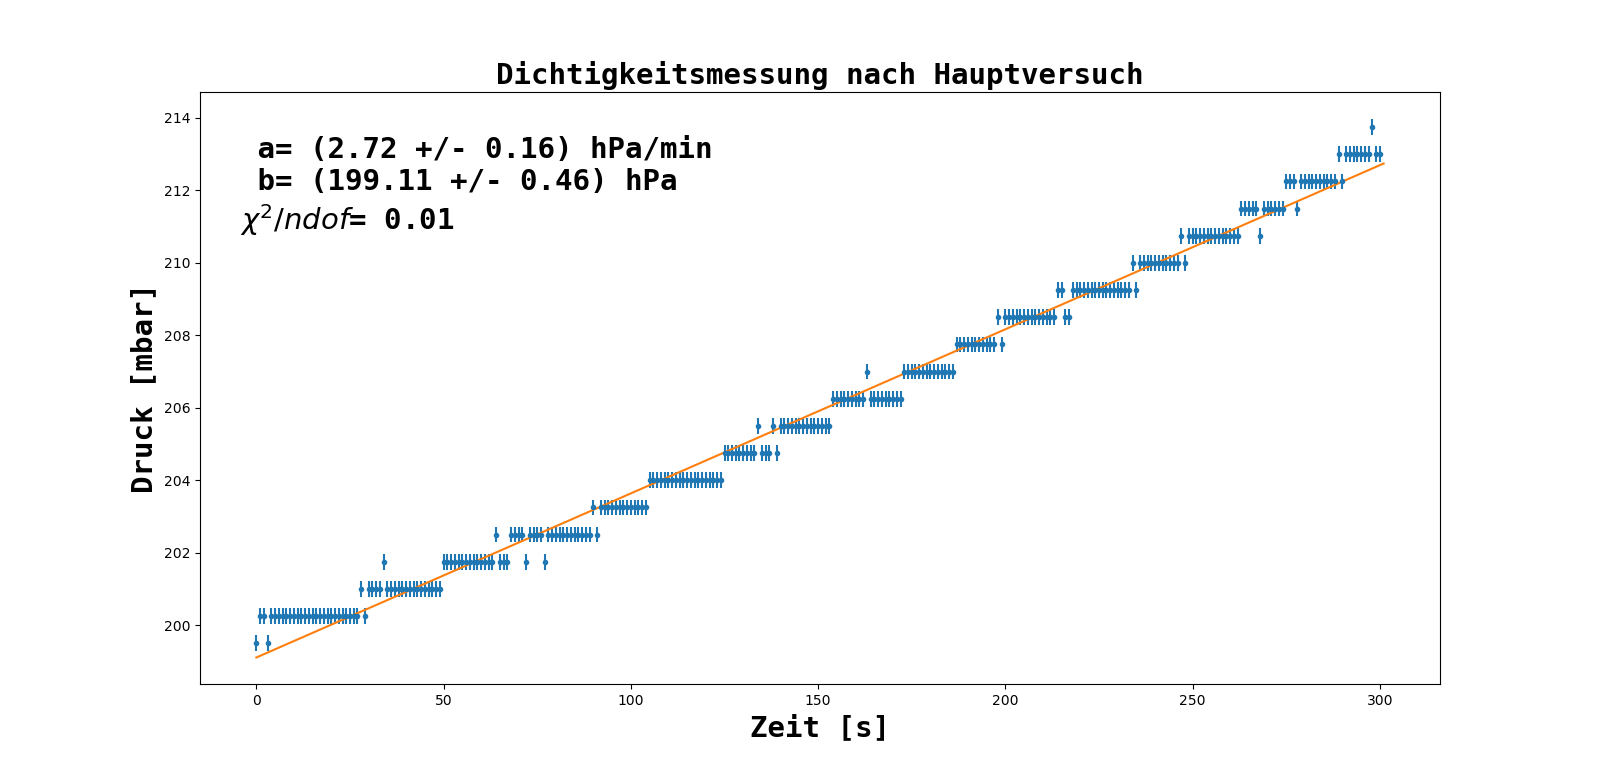
\includegraphics[width=\linewidth]{Bilder/Dichtigkeit_nachher_B.png}
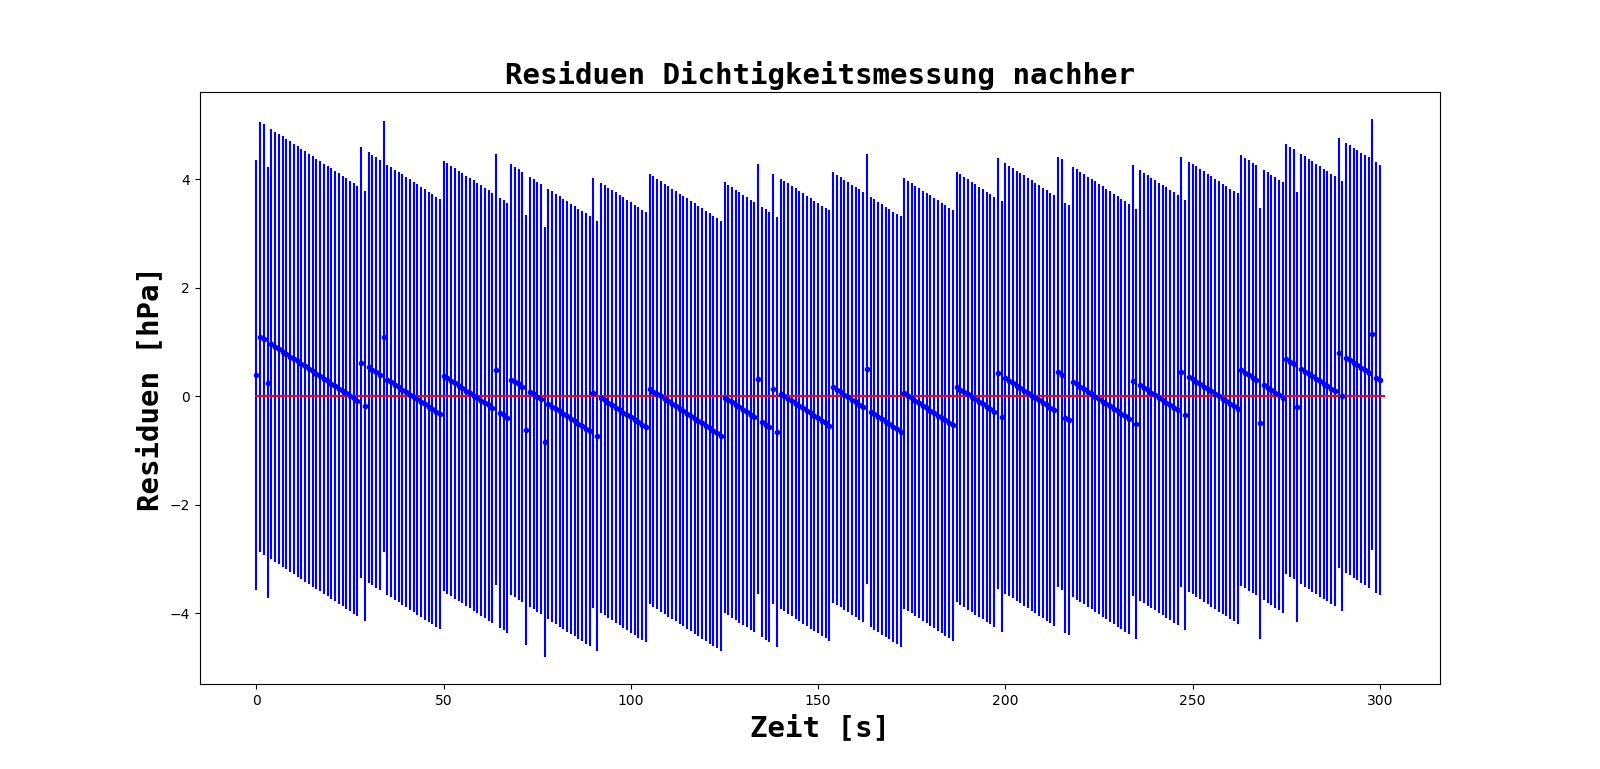
\includegraphics[width=\linewidth]{Bilder/Residuen_Dichtigkeit_nachher_B}
\caption[Dichtigkeit B nachher]{Dichtigkeit nach Haupversuch (B).}
\label{fig:DichtigkeitNachherB}
\end{figure}



\subsection{Hauptmessung}

Für die Hauptmessung wurden folgende Cassy Einstellungen verwendet:\\

\begin{tabular}{l l l}
CASSY & Kanal A & Druck p1 0-1500hPa Momentanwert\\
& Kanal B & Temperatur T1 -20C-120C Momentanwert\\
Messparameter & automatisch & Intervall 1s
\end{tabular}\\

Die Rohdaten für Druck- und die Temperaturverlauf über die Zeit finden sich für beide Verusche in Abbildung \ref{fig:RohdatenA} und \ref{fig:RohdatenB}. Fügt man diese Daten über die Zeiten zusammen erhält man die Dampfdruckkurven (siehe Abbildung \ref{fig:DampfA} und \ref{fig:DampfB}).\\


\begin{figure}[H]
\centering
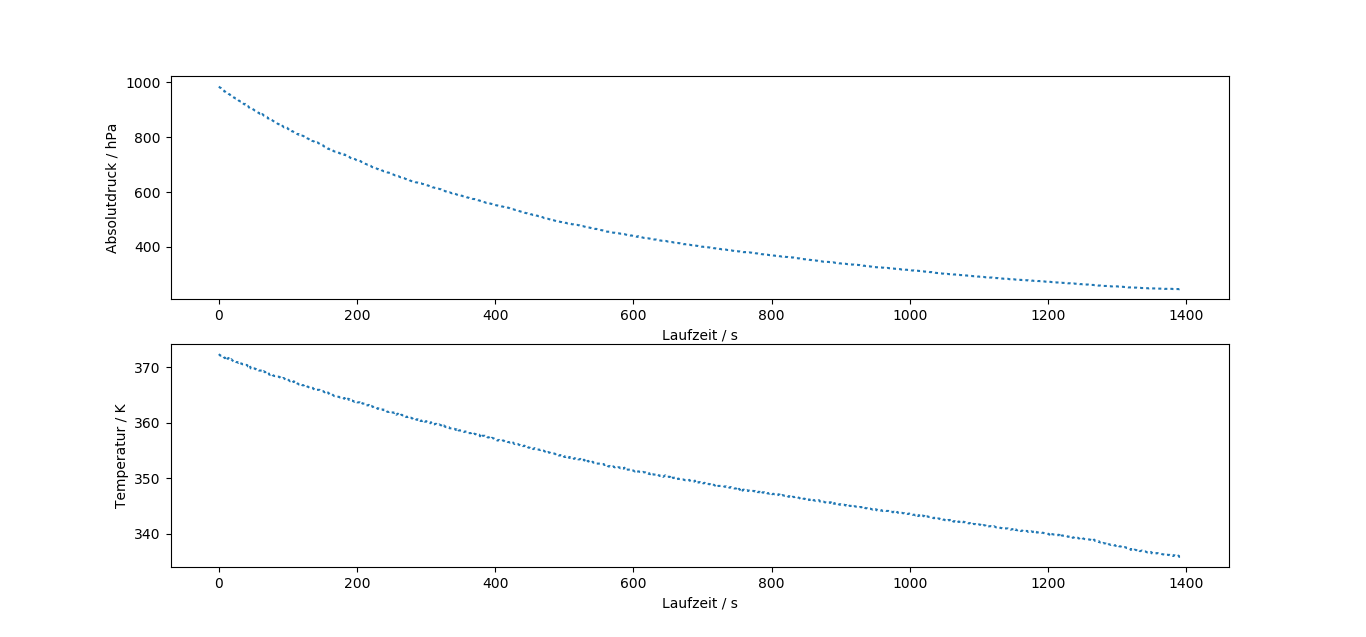
\includegraphics[width=0.9\linewidth]{Bilder/Rohdaten_HauptmessungA.png}
\caption[Rohdaten A]{Druck und Temperatur im Verlauf der Messung (A).}
\label{fig:RohdatenA}
\end{figure}


\begin{figure}[H]
\centering
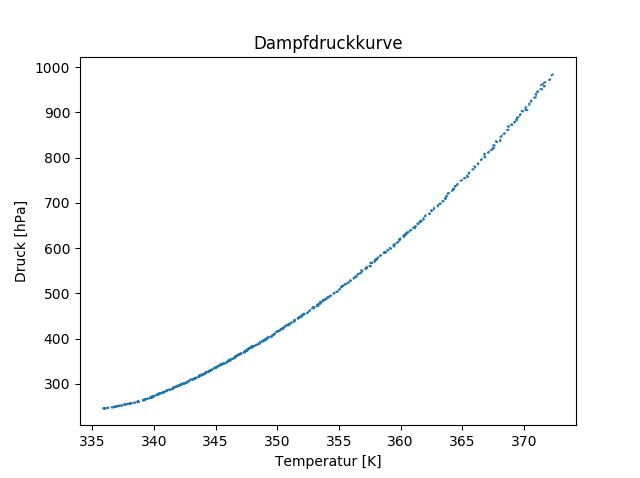
\includegraphics[width=0.8\linewidth]{Bilder/DampfdruckkurveA.png}
\caption[Dampfdruckkurve A]{Dampfdruckkurve in Versuch A}
\label{fig:DampfA}
\end{figure}

\begin{figure}[H]
\begin{center}
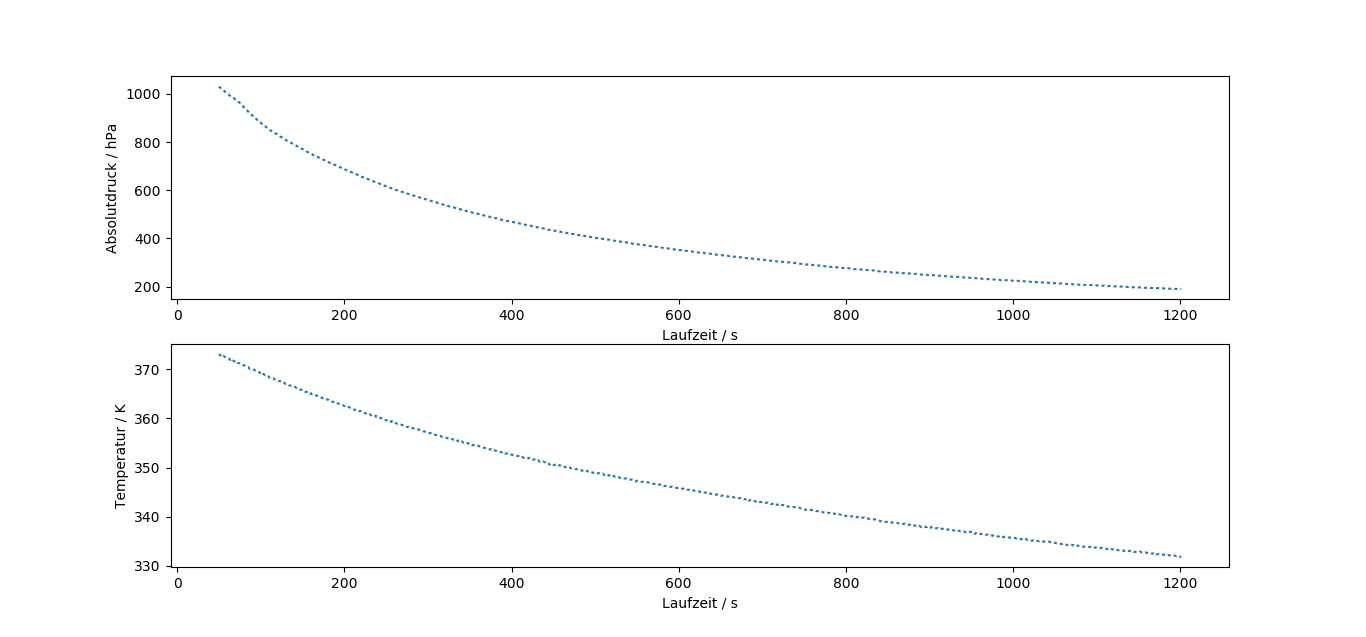
\includegraphics[width=0.9\linewidth]{Bilder/Rohdaten_HauptmessungB}
\caption[Rohdaten B]{Druck und Temperatur im Verlauf der Messung (B).}
\label{fig:RohdatenB}
\end{center}
\end{figure}

\begin{figure}[H]
\begin{center}
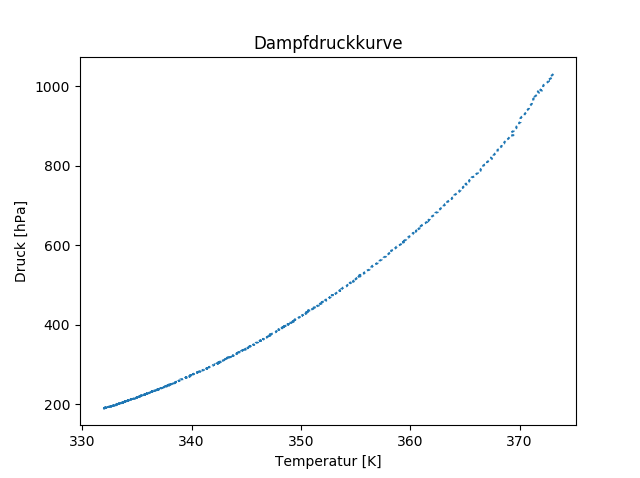
\includegraphics[width=0.8\linewidth]{Bilder/DampfdruckkurveB}
\caption[Dampfdruckkurve B]{Dampfdruckkurve in Versuch B.}
\label{fig:DampfB}
\end{center}
\end{figure}


Die statistischen Fehler der Einzelmessungen von Druck und Temperatur finden sich in den Tabellen \ref{tab:RauschenA} und \ref{tab:RauschenB}.\\
Die systematischen Fehler sind gegeben durch die Kalibrierung des Temperaturfühlers und den Fehler des Druckoffsets gegeben (vgl. Abschnitt Kalibrierung).

Trägt man nun den logarithmierten Druck gegen den Kehrwert der Temperatur auf, lässt sich der (lokale) lineare Zusammenhang gut erkennen(vgl. Abbildung \ref{fig:logA} und \ref{fig:logB}).\\

Dabei ergeben sich die statistischen und systematischen Fehler der transformierten Daten durch Fehlerfortpflanzung. Es gilt jeweils:

\begin{equation}
\sigma_{log(p/p_0)}=\frac{\sigma_p}{p} ; \quad \sigma_{1/T}=\frac{\sigma_T}{T^2}
\end{equation}

In Abbildungen \ref{fig:logA} und \ref{fig:logB} ist jeweils ein linearer Fit über den gesamten Messbereich durchgeführt worden. Betrachtet man die Residuen in Abbildung \ref{fig:logB}, so ist deutlich zu erkennen, dass der lineare Zusammenhang nicht global gültig ist ($\chi^2/dof = 28.6$). Dies ist aufgrund der Temperaturabhängigkeit von $\Lambda$ erwartet. Daher war ein ähnliches Ergebnis auch für Abbildung \ref{fig:logA} zu erwarten, dort liegen die Messwerte allerdings auch im Gesamten Bereich nah an einer Geraden ($\chi^2/dof = 0.7$).

Für die in den Abbildungen  markierten Bereich ist die lineare Anpassung in Abbildung \ref{fig:fit_2A} und \ref{fig:fit_2B} exemplarisch gezeigt.\\

\begin{figure}[H]
\begin{center}
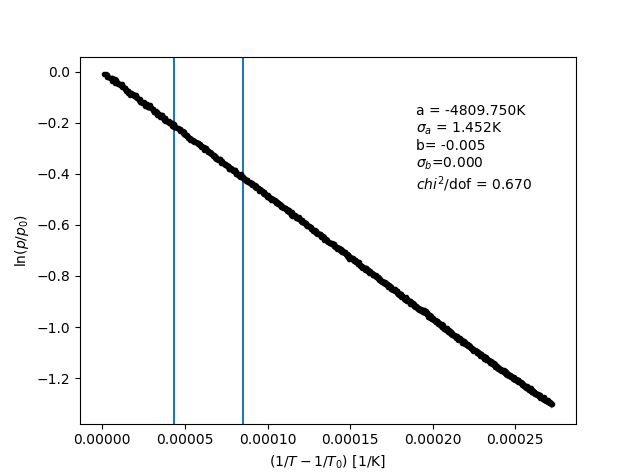
\includegraphics[width=0.75\linewidth]{Bilder/log_RohdatenA}
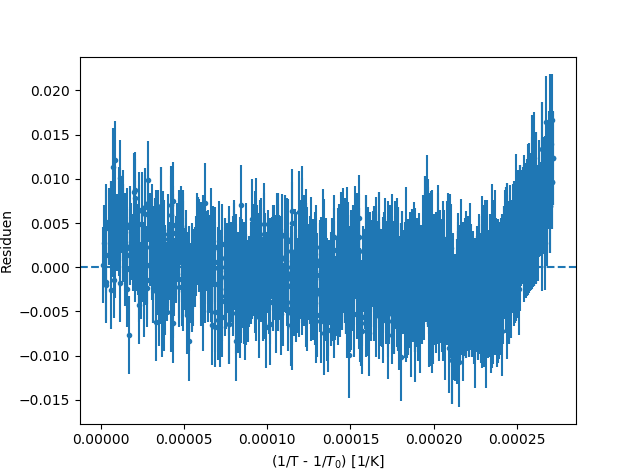
\includegraphics[width=0.75\linewidth]{Bilder/residuen_gesamt_A}
\caption[Rohdaten logarith. A]{Transformierte Daten A mit linearem Fit über Gesamten Bereich.}
\label{fig:logA}
\end{center}
\end{figure}

\begin{figure}
\centering
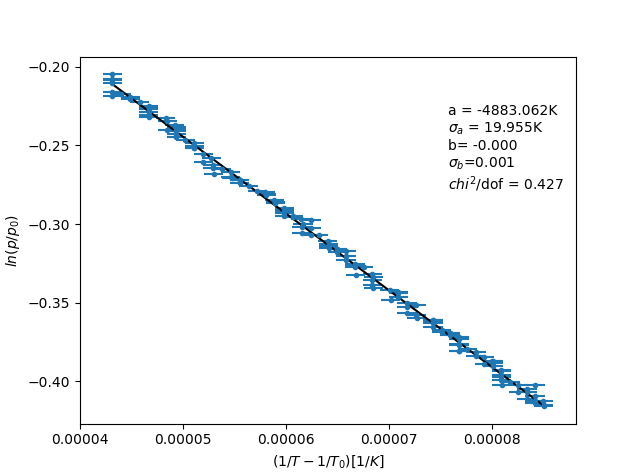
\includegraphics[width=0.8\linewidth]{Bilder/lokaler_fit_2A.png}
\includegraphics[width=0.8\linewidth]{Bilder/lokale_Residuen_2A}
\caption[Lokale Anpassung]{Lokale Anpassung im markierten Bereich (ca. 361.3K bis 367.0K) und Residuen für A. Eingezeichnet sind die stat. Fehler.}
\label{fig:fit_2A}
\end{figure}

\begin{figure}[H]
\begin{center}
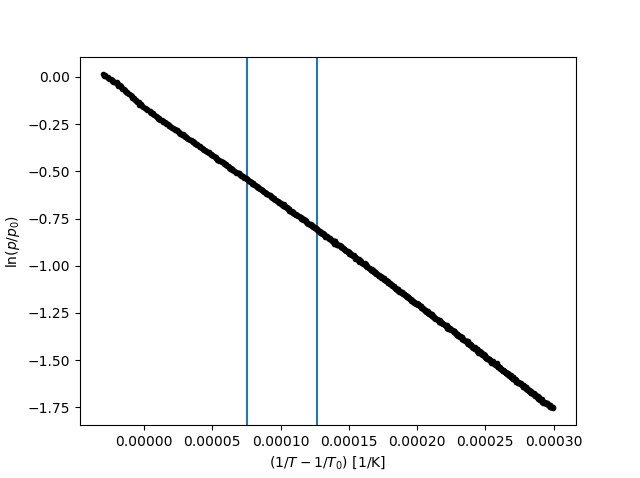
\includegraphics[width=0.9\linewidth]{Bilder/log_RohdatenB}
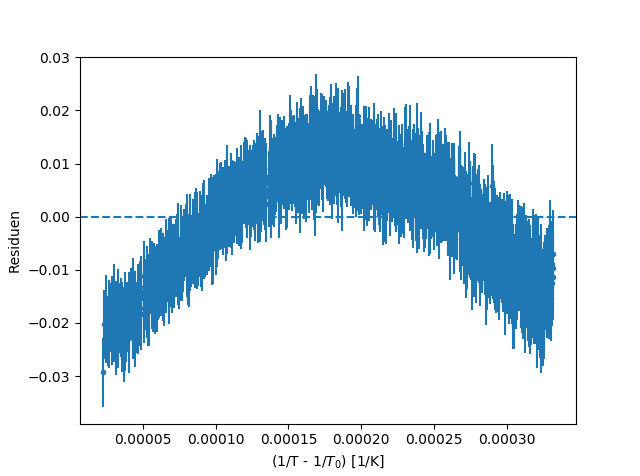
\includegraphics[width=0.9\linewidth]{Bilder/residuen_gesamt_B}
\caption[Rohdaten logarith. B]{Transformierte Daten B mit linearem Fit über Gesamten Bereich.}
\label{fig:logB}
\end{center}
\end{figure}

\begin{figure}[H]
\begin{center}
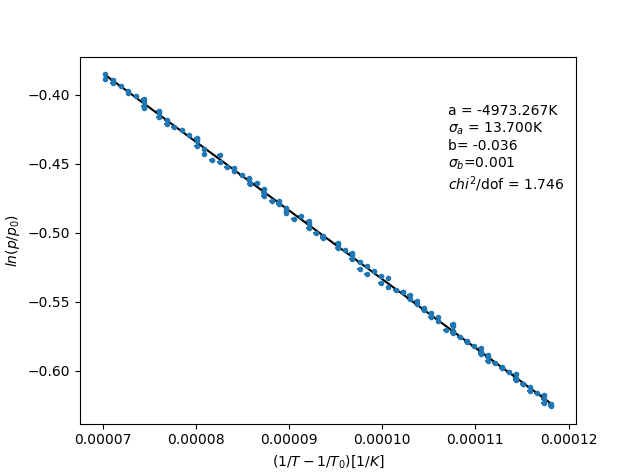
\includegraphics[width=0.9\linewidth]{Bilder/lokaler_fit_2B}\\
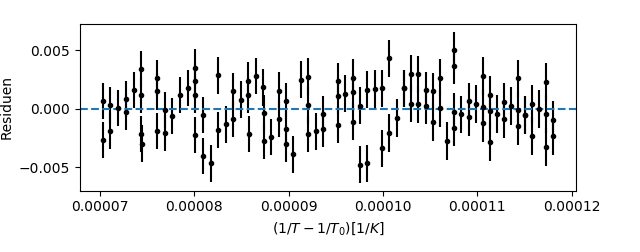
\includegraphics[width=0.9\linewidth]{Bilder/lokale_residuen_2B}
\caption[Lokale Anpassung]{Lokale Anpassung im markierten Bereich (ca. 357.1K bis 363.5K) und Residuen für B. Eingezeichnet sind die stat. Fehler.}
\label{fig:fit_2B}
\end{center}
\end{figure}


Dieses Vorgehen wurde für jeweils sechs Teilintervalle mit gleich großen Temperaturbereichen durchgeführt. Die jeweiligen Ergebnisse sind in Tabelle \ref{tab:enthalpie_A}
aufgeführt.\\


\begin{table}[H]
	\begin{tabular}{|c|c|c|c|c|}
		\hline
		\textbf{Temp. [K]} & \textbf{Steigung $\pm \sigma_{stat} \pm \sigma_{sys}$ [K]} & $\chi ^2/dof$ & \textbf{$\Lambda$ $\pm \sigma_{stat} \pm \sigma_{sys}$ [kJ/mol]} & \textbf{Abweichung} \\
		\hline
		367.0 bis 372.7 & -4917.2 $\pm$ 28.4 $\pm$ 3.6 & 0.54 & 40.88 $\pm$ 0.24 $\pm$ 0.03 & 0.3$\sigma$ \\
		\hline
		361.3 bis 367.0 & -4883.1 $\pm$ 20.0 $\pm$ 3.7 & 0.43 & 40.60 $\pm$ 0.17 $\pm$ 0.03 & 2.8$\sigma$ \\
		\hline
		355.6 bis 361.3 & -4817.7 $\pm$ 16.9 $\pm$ 3.9 & 0.05 & 40.05 $\pm$ 0.14 $\pm$ 0.03 & 8.8$\sigma$ \\
		\hline
		349.9 bis 355.6 & -4814.2 $\pm$ 14.8 $\pm$ 4.1 & 0.06 & 40.03 $\pm$ 0.12 $\pm$ 0.03 & 12.2$\sigma$ \\
		\hline
		344.2 bis 349.9 & -4867.6 $\pm$ 12.8 $\pm$ 4.5 & 0.08 & 40.47 $\pm$ 0.11 $\pm$ 0.04 & 12.2$\sigma$ \\
		\hline
		338.5 bis 344.2 & -4505.3 $\pm$ 10.7 $\pm$ 4.7 & 0.07 & 37.46 $\pm$ 0.09 $\pm$ 0.04 & 48.1$\sigma$ \\
		\hline 
	\end{tabular}\\		
\\

	\begin{tabular}{|c|c|c|c|c|}
		\hline
		\textbf{Temp. [K]} & \textbf{Steigung $\pm \sigma_{stat} \pm \sigma_{sys}$ [K]} & $\chi ^2/dof$ & \textbf{$\Lambda$ $\pm \sigma_{stat} \pm \sigma_{sys}$ [kJ/mol]} & \textbf{Abweichung} \\
		\hline
		363.4 bis 369.7 & -4981.9 $\pm$ 18.6 $\pm$ 4.9 & 0.11 & 41.42 $\pm$ 0.15 $\pm$ 0.04 & 2.9$\sigma$ \\
		\hline
		357.1 bis 363.4 & -4973.6 $\pm$ 13.7 $\pm$ 5.1 & 0.10 & 41.35 $\pm$ 0.11 $\pm$ 0.04 & 0.9$\sigma$ \\
		\hline
		350.8 bis 357.1 & -5095.7 $\pm$ 15.9 $\pm$ 5.5 & 0.02 & 42.37 $\pm$ 0.13 $\pm$ 0.05 & 5.9$\sigma$ \\
		\hline
		344.5 bis 350.8 & -5366.2 $\pm$ 12.6 $\pm$ 6.2 & 0.02 & 44.61 $\pm$ 0.10 $\pm$ 0.05 & 24.0$\sigma$ \\
		\hline
		338.2 bis 344.5 & -5411.0 $\pm$ 12.4 $\pm$ 7.0 & 0.03 & 44.99 $\pm$ 0.10 $\pm$ 0.06 & 24.4$\sigma$ \\
		\hline
		331.9 bis 338.2 & -5484.1 $\pm$ 11.2 $\pm$ 8.2 & 0.04 & 45.59 $\pm$ 0.09 $\pm$ 0.07 & 27.8$\sigma$ \\
		\hline
	\end{tabular}



	\caption{Ergebnisse für die Verdampfungsenthalpie nach Temperatur für Versuch A (oben) und Versuch B (unten).}
	\label{tab:enthalpie_A}
\end{table}

Die Verdampfungsenthalpie ist dabei gegeben durch $\Lambda=-a \cdot R$ und der statistische Fehler ergibt sich mittels Fehlerfortpflanzung zu $\sigma_{\Lambda, stat}=R \cdot \sigma_{a,stat}$.\\
Um einen systematischen Fehler abzuschätzen eignet sich die Verschiebemethode. Dazu werden die Messpunkte mit ihren statistischen Fehlern um die systematischen Fehler verschoben, einmal nach oben und einmal nach unten,   \\

\begin{equation}
	ln(p/p_0)_{i, verschoben} = ln(p/p_0)_{i} - \sigma _{ln(p/p_0), syst}
\end{equation}
bzw.
\begin{equation}
	ln(p/p_0)_{i, verschoben} = ln(p/p_0)_{i} + \sigma _{ln(p/p_0), syst}
\end{equation}

und man wiederholt jeweils die lineare Regression. So erhält man zwei neue Werte $\Lambda_{p,-}$ bzw. $\Lambda_{p,+}$ für die Verdampfungsenthalpie. Der Teil des systematischen Fehlers, der von der Druckmessung herrührt, ist dann der Mittelwert der Abweichungen:
\begin{equation}
	\Delta \Lambda _{syst,p} = ( |\Lambda_{p,-}-\Lambda| + |\Lambda_{p,+} - \Lambda|)/2 .
\end{equation}

Den Beitrag durch den systematischen Temperaturfehler erhält man ebenfalls durch die Verschiebemethode. Der systematische Gesamtfehler ergibt sich dann durch quadratische Addition.\\

\begin{equation}
\Delta \Lambda_{syst}^2 = \Delta \Lambda_{syst,p}^2 + \Delta \Lambda_{syst,T}^2
\end{equation}

Da $\Lambda$ temperaturabhängig ist, muss der zur Messung passende Literaturwert erst noch bestimmt werden. Dazu haben wir als lineare Approximation eine Gerade durch die Literaturwerte zu 60C und 100C gelegt. Abbildung \ref{fig:LiteraturwertLambda} zeigt die Literaturwerte (60C, 80C, 100C) als blaue Punkte und die lineare Näherung als rote Linie. Es lässt sich leicht erkennen, dass die Näherung in diesem Temperaturbereich gut funktioniert. Daher wird mit dieser gerechnet und diese ist auch in die Ergebnisplots eingezeichnet. \\
In Abb. \ref{fig:EntTempA} findet sich die Auftragung der verschiedenen Werte von $\Lambda$ bei den entsprechenden Temperaturen. In Abb. \ref{fig:EntTempB} findet sich die selbe Darstellung für Aufbau B.\\

Es fällt auf, dass bei beiden Versuchen die zeitlich ersten Werte im Rahmen ihrer Fehler relativ gut mit dem Literaturwert übereinstimmen (Jeweils die zwei Werte rechts in den Abbildungen \ref{fig:EntTempA} und \ref{fig:EntTempB}).
Allerdings sind die restlichen Werte für $\Lambda$ in Aufbau A deutlich kleiner als die Literaturwerte und auch unter Berücksichtigung der Fehler nicht mehr mit dem Literaturwert vereinbar. Der Wert links in der Abbildung ist zeitlich gesehen der letzte Wert. Eine zumindest für diesen Wert naheliegende Erklärung ist, dass das Wasser zu diesem Zeitpunkt bereits nicht mehr am Sieden war. Für die übrigen Abweichungen liegen keine konkreten Erklärungen vor, am wahrscheinlichsten erscheint hier ein nicht näher bekanntes Problem mit dem Aufbau. \\
Ähnlich verhält es sich für B, hier sind die übrigen Werte jedoch deutlich zu groß.\\
Es ist naheliegend, dass die angegebenen Unsicherheiten um etwa eine Größenordnung zu klein sind, allerdings ist uns nicht klar woran dies liegt.\\
Man beachte, dass ein zu großer Druck (z.B. durch den Partialdruck zusätzlich eingeschlossener Luft) für eine betragsmäßig größere Steigung sorgt und infolge dessen zu einem erhöhten Wert für $\Lambda$ führt.
Die Abweichung nimmt mit zunehmender Messdauer (entspricht kleinerer Temperatur) immer mehr zu. Berücksichtigt man noch die zweite Dichtigkeitsmessung, welche deutlich schlechter als die erste ausgefallen ist, lässt sich zusammenfassend sagen, dass Aufbau B möglicherweise doch zu undicht war und während des Versuches eine ausreichend große Menge Luft in den Kolben eingedrungen ist und somit der gemessene Druck zunehmend größer als der tatsächliche Dampfdruck des Wassers wurde.\\





\begin{figure}[H]
\begin{center}
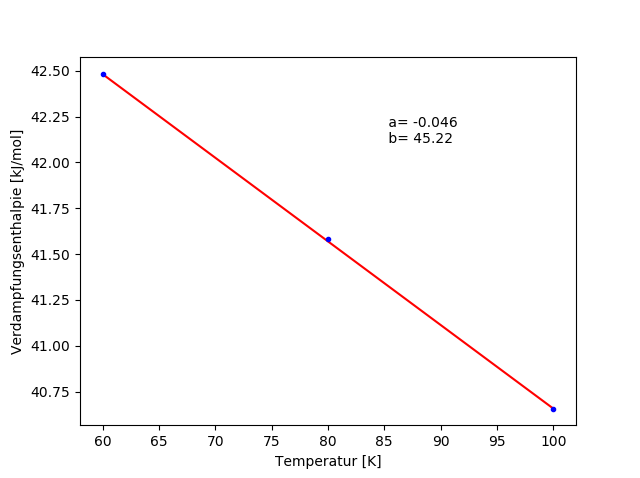
\includegraphics[scale=0.9]{Bilder/Lambda_Literaturwert_fit.png}
\caption[Literaturwerte für $\Lambda$ in Abhängigkeit von der Temperatur]{Literaturwerte für $\Lambda$ in Abhängigkeit von der Temperatur}
\label{fig:LiteraturwertLambda}
\end{center}
\end{figure}


\begin{figure}
\begin{center}
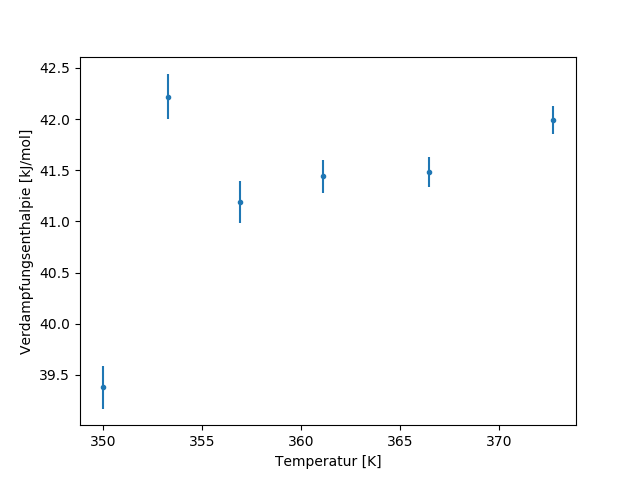
\includegraphics[width=0.8\linewidth]{Bilder/Enthalpie_gegen_TempA}
\caption{Versuch A: Enthalpie mit stat. und syst. Fehlern gegen Temperatur und Literaturwerte (Gerade).}
\label{fig:EntTempA}
\end{center}
\end{figure}
\begin{figure}[H]
\begin{center}
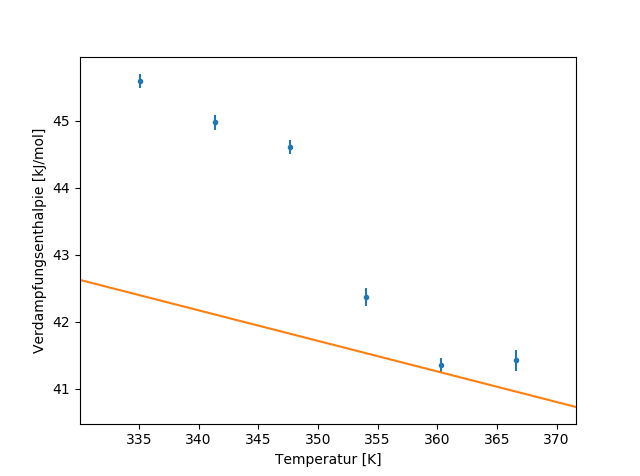
\includegraphics[width=0.8\linewidth]{Bilder/Enthalpie_gegen_TempB}
\caption{Versuch B: Enthalpie mit stat. und syst. Fehlern gegen Temperatur und Literaturwerte (Gerade).}
\label{fig:EntTempB}
\end{center}
\end{figure}






\section{Fazit}
Beiden Gruppen ist es nicht gelungen ein zufriedenstellendes Ergebnis zu erzielen. Nur zu Beginn der Messung stimmen wenige gemessene Werte im Rahmen der Messunsicherheit mit den Literaturwerten überein. Die übrigen Werte sind entweder viel kleiner (A) oder viel zu groß (B).\\
Die Ursache für diese Abweichungen liegt wahrscheinlich im sehr empfindlichen Aufbau des Versuchs, welcher  während oder kurz vor der Hauptmessung gestört wurde. Dadurch ist die vernachlässigbare Undichtigkeit nicht mehr gewährleistet gewesen und es kommt zu den größtenteils massiven Abweichungen.


\end{document}
